% Options for packages loaded elsewhere
\PassOptionsToPackage{unicode}{hyperref}
\PassOptionsToPackage{hyphens}{url}
\PassOptionsToPackage{dvipsnames,svgnames,x11names}{xcolor}
%
\documentclass[
  11pt,
  dvipsnames,enabledeprecatedfontcommands]{scrartcl}
\usepackage{amsmath,amssymb}
\usepackage{lmodern}
\usepackage{iftex}
\ifPDFTeX
  \usepackage[T1]{fontenc}
  \usepackage[utf8]{inputenc}
  \usepackage{textcomp} % provide euro and other symbols
\else % if luatex or xetex
  \usepackage{unicode-math}
  \defaultfontfeatures{Scale=MatchLowercase}
  \defaultfontfeatures[\rmfamily]{Ligatures=TeX,Scale=1}
\fi
% Use upquote if available, for straight quotes in verbatim environments
\IfFileExists{upquote.sty}{\usepackage{upquote}}{}
\IfFileExists{microtype.sty}{% use microtype if available
  \usepackage[]{microtype}
  \UseMicrotypeSet[protrusion]{basicmath} % disable protrusion for tt fonts
}{}
\usepackage{xcolor}
\usepackage{graphicx}
\makeatletter
\def\maxwidth{\ifdim\Gin@nat@width>\linewidth\linewidth\else\Gin@nat@width\fi}
\def\maxheight{\ifdim\Gin@nat@height>\textheight\textheight\else\Gin@nat@height\fi}
\makeatother
% Scale images if necessary, so that they will not overflow the page
% margins by default, and it is still possible to overwrite the defaults
% using explicit options in \includegraphics[width, height, ...]{}
\setkeys{Gin}{width=\maxwidth,height=\maxheight,keepaspectratio}
% Set default figure placement to htbp
\makeatletter
\def\fps@figure{htbp}
\makeatother
\setlength{\emergencystretch}{3em} % prevent overfull lines
\providecommand{\tightlist}{%
  \setlength{\itemsep}{0pt}\setlength{\parskip}{0pt}}
\setcounter{secnumdepth}{5}
\newlength{\cslhangindent}
\setlength{\cslhangindent}{1.5em}
\newlength{\csllabelwidth}
\setlength{\csllabelwidth}{3em}
\newlength{\cslentryspacingunit} % times entry-spacing
\setlength{\cslentryspacingunit}{\parskip}
\newenvironment{CSLReferences}[2] % #1 hanging-ident, #2 entry spacing
 {% don't indent paragraphs
  \setlength{\parindent}{0pt}
  % turn on hanging indent if param 1 is 1
  \ifodd #1
  \let\oldpar\par
  \def\par{\hangindent=\cslhangindent\oldpar}
  \fi
  % set entry spacing
  \setlength{\parskip}{#2\cslentryspacingunit}
 }%
 {}
\usepackage{calc}
\newcommand{\CSLBlock}[1]{#1\hfill\break}
\newcommand{\CSLLeftMargin}[1]{\parbox[t]{\csllabelwidth}{#1}}
\newcommand{\CSLRightInline}[1]{\parbox[t]{\linewidth - \csllabelwidth}{#1}\break}
\newcommand{\CSLIndent}[1]{\hspace{\cslhangindent}#1}
%\documentclass{article}

% %packages
\usepackage{booktabs}
%\usepackage[left]{showlabels}
\usepackage{multirow}
\usepackage{subcaption}
\usepackage{wrapfig}
\usepackage{graphicx}
\usepackage{longtable}
\usepackage{ragged2e}
\usepackage{etex}
%\usepackage{yfonts}
\usepackage{marvosym}
\usepackage[notextcomp]{kpfonts}
\usepackage{nicefrac}
\newcommand*{\QED}{\hfill \footnotesize {\sc Q.e.d.}}
\usepackage{floatrow}
\usepackage{multicol}

\usepackage{setspace}
\usepackage[pagewise]{lineno}

\usepackage[textsize=footnotesize]{todonotes}
\newcommand{\ali}[1]{\todo[color=gray!40]{\textbf{Alicja:} #1}}
\newcommand{\mar}[1]{\todo[color=blue!40]{#1}}
\newcommand{\raf}[1]{\todo[color=olive!40]{#1}}

%\linespread{1.5}
\newcommand{\indep}{\!\perp \!\!\! \perp\!}


\setlength{\parindent}{10pt}
\setlength{\parskip}{1pt}


%language
%\usepackage{times}
\usepackage{mathptmx}
\usepackage[scaled=0.86]{helvet}
\usepackage{t1enc}
%\usepackage[utf8x]{inputenc}
%\usepackage[polish]{babel}
%\usepackage{polski}




%AMS
\usepackage{amsfonts}
\usepackage{amssymb}
\usepackage{amsthm}
\usepackage{amsmath}
\usepackage{mathtools}

\usepackage{geometry}
 \geometry{a4paper,left=35mm,top=20mm,}


%environments
\newtheorem{fact}{Fact}


% allow page breaks in equations
\allowdisplaybreaks


%abbreviations
\newcommand{\ra}{\rangle}
\newcommand{\la}{\langle}
\newcommand{\n}{\neg}
\newcommand{\et}{\wedge}
\newcommand{\jt}{\rightarrow}
\newcommand{\ko}[1]{\forall  #1\,}
\newcommand{\ro}{\leftrightarrow}
\newcommand{\exi}[1]{\exists\, {_{#1}}}
\newcommand{\pr}[1]{\ensuremath{\mathsf{P}(#1)}}
\newcommand{\ppr}[2]{\ensuremath{\mathsf{P}^{#1}(#2)}}
\newcommand{\cost}{\mathsf{cost}}
\newcommand{\benefit}{\mathsf{benefit}}
\newcommand{\ut}{\mathsf{ut}}

\newcommand{\odds}{\mathsf{Odds}}
\newcommand{\ind}{\mathsf{Ind}}
\newcommand{\nf}[2]{\nicefrac{#1\,}{#2}}
\newcommand{\R}[1]{\texttt{#1}}
\newcommand{\prr}[1]{\mbox{$\mathtt{P}_{prior}(#1)$}}
\newcommand{\prp}[1]{\mbox{$\mathtt{P}_{posterior}(#1)$}}



\newtheorem{q}{\color{blue}Question}
\newtheorem{lemma}{Lemma}
\newtheorem{theorem}{Theorem}
\newtheorem{corollary}{Corollary}[fact]


%technical intermezzo
%---------------------

\newcommand{\intermezzoa}{
	\begin{minipage}[c]{13cm}
	\begin{center}\rule{10cm}{0.4pt}



	\tiny{\sc Optional Content Starts}
	
	\vspace{-1mm}
	
	\rule{10cm}{0.4pt}\end{center}
	\end{minipage}\nopagebreak 
	}


\newcommand{\intermezzob}{\nopagebreak 
	\begin{minipage}[c]{13cm}
	\begin{center}\rule{10cm}{0.4pt}

	\tiny{\sc Optional Content Ends}
	
	\vspace{-1mm}
	
	\rule{10cm}{0.4pt}\end{center}
	\end{minipage}
	}
	
	
%--------------------






















\newtheorem*{reply*}{Reply}
\usepackage{enumitem}
\newcommand{\question}[1]{\begin{enumerate}[resume,leftmargin=0cm,labelsep=0cm,align=left]
\item #1
\end{enumerate}}

\usepackage{float}

% \setbeamertemplate{blocks}[rounded][shadow=true]
% \setbeamertemplate{itemize items}[ball]
% \AtBeginPart{}
% \AtBeginSection{}
% \AtBeginSubsection{}
% \AtBeginSubsubsection{}
% \setlength{\emergencystretch}{0em}
% \setlength{\parskip}{0pt}






\usepackage[authoryear]{natbib}

%\bibliographystyle{apalike}



\usepackage{tikz}
\usetikzlibrary{positioning,shapes,arrows}

\ifLuaTeX
  \usepackage{selnolig}  % disable illegal ligatures
\fi
\IfFileExists{bookmark.sty}{\usepackage{bookmark}}{\usepackage{hyperref}}
\IfFileExists{xurl.sty}{\usepackage{xurl}}{} % add URL line breaks if available
\urlstyle{same} % disable monospaced font for URLs
\hypersetup{
  pdftitle={Awareness Growth in Bayesian Networks},
  colorlinks=true,
  linkcolor={Maroon},
  filecolor={Maroon},
  citecolor={Blue},
  urlcolor={blue},
  pdfcreator={LaTeX via pandoc}}

\title{Awareness Growth in Bayesian Networks}
\author{}
\date{\vspace{-2.5em}July 28, 2022}

\begin{document}
\maketitle

\doublespace

\emph{Wordcount (including footnotes)}: 5,392

\begin{abstract}
We examine different counterexamples to Reverse Bayesianism, a popular theory 
that addresses the problem of awareness growth. We agree with the general skepticism toward Reverse Bayesianism, but submit that the problem of awareness growth cannot be tackled in an algorithmic manner, because subject-matter, structural assumptions need to be made explicit. Thanks to their ability to express probabilistic dependencies, we illustrate how Bayesian networks can help to model awareness growth in the Bayesian framework. 
\end{abstract}

\doublespace
\linenumbers

\hypertarget{introduction}{%
\section{Introduction}\label{introduction}}

Learning is modeled in the Bayesian framework by the rule of
conditionalization. This rule posits that the agent's new degree of
belief in a proposition \(H\) after a learning experience \(E\) should
be the same as the agent's old degree of belief in \(H\) conditional on
\(E\). That is, \[\ppr{E}{H}=\pr{H \vert E},\] where \(\pr{}\)
represents the agent's old degree of belief (before the learning
experience \(E\)) and \(\ppr{E}{}\) represents the agent's new degree of
belief (after the learning experience \(E\)).

Both \(E\) and \(H\) belong to the agent's algebra of propositions. This
algebra models the agent's awareness state, the propositions taken to be
live possibilities. Conditionalization never modifies the algebra and
thus makes it impossible for an agent to learn something they have never
thought about. Even before learning about \(E\), the agent must already
have assigned a degree of belief to any proposition conditional on
\(E\). This picture commits the agent to the specification of their
`total possible future experience' (Howson, 1976), as though learning
was confined to an `initial prison' (Lakatos, 1968).

But, arguably, the learning process is more complex than what
conditionalization allows. Not only do we learn that some propositions
that we were entertaining are true or false, but we may also learn new
propositions that we did not entertain before. Or we may entertain new
propositions---without necessarily learning that they are true or
false---and this change in awareness may in turn change what we already
believe. How should this more complex learning process be modeled by
Bayesianism? Call this the problem of awareness growth.

The algebra of propositions need not be so narrowly construed that it
only contains propositions that are presently under consideration. The
algebra may also contain propositions which, though outside the agent's
present consideration, are still the object, perhaps implicitly, of
certain dispositions to believe.\footnote{Roussos (2021) notes that, for
  the sake of clarity, the problem of awareness growth should only
  address propositions which agents are \emph{truly} unaware of (say new
  scientific theories), not propositions that were temporarily forgotten
  or set aside. This is a helpful clarification to keep in mind,
  although the recent literature on the topic does not make a sharp a
  distinction between true unawareness and temporary unawareness.} But
even this expanded algebra will have to be revised sooner or later. The
algebra of propositions could in principle contain anything that could
possibly be conceived, expressed, thought of. Such a rich algebra would
not need to change at any point, but this is an implausible model of
ordinary agents with bounded resources such as ourselves.

Critics of Bayesianism and sympathizers alike have been discussing the
problem of awareness growth under different names for quite some time,
at least since the eighties. This problem arises in a number of
different contexts, for example, new scientific theories (Chihara, 1987;
Earman, 1992; Glymour, 1980), language changes and paradigm shifts
(Williamson, 2003), and theories of induction (Zabell, 1992). A proposal
that has attracted considerable scholarly attention in recent years is
Reverse Bayesianism (Bradley, 2017; Karni \& Vierø, 2015; Wenmackers \&
Romeijn, 2016). The idea is to model awareness growth as a change in the
algebra while ensuring that the proportions of probabilities of the
propositions shared between the old and new algebra remain the same in a
sense to be specified.

Let \(\mathcal{F}\) be the initial algebra of propositions and let
\(\mathcal{F}^+\) the algebra after the agent's awareness state has
grown. Both algebras contain the contradictory and tautologous
propositions \(\perp\) and \(\top\), and they are closed under
connectives such as disjunction \(\vee\), conjunction \(\wedge\) and
negation \(\neg\). Denote by \(X\) and \(X^+\) the subsets of these
algebras that contain only basic propositions, namely those without
connectives. \textbf{Reverse Bayesianism} posits that the ratio of
probabilities for any basic propositions \(A\) and \(B\) in both \(X\)
and \(X^+\)---the basic propositions shared by the old and new
algebra---remain constant through the process of awareness growth:
\[\frac{\pr{A}}{\pr{B}} = \frac{\ppr{+}{A}}{\ppr{+}{B}},\] where
\(\pr{}\) represents the agent's degree of belief before awareness
growth and \(\ppr{+}{}\) represents the agent's degree of belief after
awareness growth.

Reverse Bayesianism is an elegant theory that manages to cope with a
seemingly intractable problem. As the awareness state of an an agent
grows, the agent would prefer not to throw away completely the epistemic
work they have done previously. The agent may desire to retain as much
of their old degrees of beliefs as possible. Reverse Bayesianism
provides a simple recipe to do that. It also coheres with the
conservative spirit of Bayesian conditionalization which preserves the
old probability distribution conditional on what is learned.

Unfortunately, Reverse Bayesianism does not deliver the intuitive
results in all cases. There is no shortage of counterexamples against it
in the recent philosophical literature (Mathani, 2020; Steele \&
Stefánsson, 2021). In addition, attempts to extent traditional arguments
in defense of Bayesian conditionalization to the case of awareness
growth seem to hold little promise (Pettigrew, forthcoming). If the
consensus in the literature is that Reverse Bayesianism is not the right
theory of awareness growth, what theory (if any) should replace it?

Here we offer a diagnosis of what is wrong with Reverse Bayesianism and
outline an alternative proposal. The problem of awareness growth---we
hold---cannot be tackled in an algorithmic manner because subject-matter
assumptions, both probabilistic and structural, need to be made
explicit. So any theory of awareness growth cannot be a purely formal
theory. This does not mean, however, we should give up on probability
theory altogether. Thanks to their ability to express probabilistic
dependencies, Bayesian networks can help to model awareness growth in
the Bayesian framework. We illustrate this claim as we examine different
counterexamples to Reverse Bayesianism.

\hypertarget{steele-and-stefuxe1nssons-examples}{%
\section{Steele and Stefánsson's
Examples}\label{steele-and-stefuxe1nssons-examples}}

\label{sec:counterexamples}

In this section, we rehearse two of the counterexamples to Reverse
Bayesianism by Steele \& Stefánsson (2021). One example targets
awareness expansion and the other awareness refinement. A precise
definition of expansion can be tricky to provide, but a rough
characterization will suffice for now. Suppose, as is customary,
propositions are interpreted as sets of possible worlds, where the set
of all possible worlds is the possibility space. Awareness expansion
occurs when a new proposition is added to the algebra and its
interpretation includes possible worlds not in the original possibility
space. So the addition of the new proposition causes the possibility
space to expand. By contrast, awareness refinement (roughly) occurs when
the new proposition added to the algebra induces a more fine-grained
partition of the possibility space.

The most straightforward case of \emph{awareness expansion} occurs when
you become aware of a new explanation for the evidence at your disposal
which you had not considered before. This can happen in many fields of
inquiry: medicine, law, science, everyday affairs. Here is a scenario by
Steele \& Stefánsson (2021):

\begin{quote}
\textsc{Friends}: Suppose you happen to see your partner enter your best
friend's house on an evening when your partner had told you she would
have to work late. At that point, you become convinced that your partner
and best friend are having an affair, as opposed to their being warm
friends or mere acquaintances. You discuss your suspicion with another
friend of yours, who points out that perhaps they were meeting to plan a
surprise party to celebrate your upcoming birthday---a possibility that
you had not even entertained. (Steele \& Stefánsson, 2021, sec. 5,
Example 2)
\end{quote}

\doublespace

\noindent Initially, the algebra contained the hypotheses `my partner
and my best friend met to have an affair' (\textit{affair}) and `my
partner and my best friend met as friends' (\textit{friends}). These
were the only explanations you considered for the fact that your partner
and your best friend met one night without telling you. But, when the
algebra changes, a new hypothesis is added which you had not considered
before: your partner and your best friends met to plan a surprise party
for your upcoming birthday (\textit{surprise}).

This change in the algebra is not innocuous. At first, the hypothesis
\textit{affair} seems more likely than \textit{friends} because the
former seems a better explanation than the latter for the secretive
behavior of your partner and best friend.\footnote{This assumes that the
  prior probabilities of the two hypotheses were not strongly skewed in
  one direction. If you were initially nearly certain your partner could
  not possibly have an affair with your best friend, the fact they
  behaved secretively or lied to you should not affect that much the
  probability of the two hypotheses.} But when the new hypothesis
\textit{surprise} is added, things change: \textit{surprise} now seems a
better explanation overall and thus more likely than \textit{affair}.
And since \textit{surprise} implies \textit{friends}, the latter must be
more likely than \textit{affair}. This conclusion violates Reverse
Bayesianism since the ratio of the probabilities of \textit{friends} and
\textit{affair} has changed before and after awareness expansion.

Steele \& Stefánsson note that a quick fix is available. It is
reasonable to suppose that no change in the probabilities should occur
so long as we confine ourselves to the old probability space. With this
in mind, consider the following condition, called
\textbf{Awareness Rigidity}: \[\ppr{+}{A \vert T^*}=\pr{A},\] where
\(T^*\) corresponds to a proposition that picks out, from the vantage
point of the new awareness state, the entire possibility space
\emph{before} the episode of awareness growth. Awareness rigidity posits
that, once a suitable proposition \(T^*\) is identified, the old
probability assignments remain unchanged conditional on \(T^*\). In our
running example, \(\neg\textit{surprise}\) is the suitable proposition
\(T^*\): \emph{that} there were was no surprise party in the making
picks out the original possibility space. Conditional on
\(\neg\textit{surprise}\), no probability assignment should change,
including the probability of \textit{affair}. This is the intended
result.

But this is not the end of the story. Steele \& Stefánsson go on to show
that Awareness Rigidity does not hold in other cases, what they call
\emph{awareness refinement}. As noted before, these are cases in which
the new proposition induces a more fine-grained partition of the
possibility space. Consider this scenario:

\begin{quote}
\textsc{Movies}: Suppose you are deciding whether to see a movie at your
local cinema. You know that the movie's predominant language and genre
will affect your viewing experience. The possible languages you consider
are French and German and the genres you consider are thriller and
comedy. But then you realise that, due to your poor French and German
skills, your enjoyment of the movie will also depend on the level of
difficulty of the language. Since it occurs to you that the owner of the
cinema is quite simple-minded, you are, after this realisation, much
more confident that the movie will have low-level language than
high-level language. Moreover, since you associate low-level language
with thrillers, this makes you more confident than you were before that
the movie on offer is a thriller as opposed to a comedy. (Steele \&
Stefánsson, 2021, sec. 5, Example 3)
\end{quote}

\doublespace

\noindent You initially categorized movies by just language and genre,
and then you refined your categorization by adding another variable,
level of difficulty. Without considering language difficulty, you
assigned the same probability to the hypotheses \textit{thriller} and
\textit{comedy}. But learning that the owner was simple-minded made you
think that the level of linguistic difficulty must be low and the movie
most likely a thriller rather than a comedy (perhaps because thrillers
are simpler---linguistically---than comedies). Since the probability of
\textit{thriller} goes up, this scenario violates (against Reverse
Bayesianism) the condition
\(\frac{\pr{\textit{thriller}}}{\pr{\textit{comedy}}}=\frac{\ppr{+}{\textit{thriller}}}{\ppr{+}{\textit{Comedy}}}\).
For the same reason, it also violates (against Awareness Rigidity) the
condition
\(\pr{\textit{thriller}}=\ppr{+}{\textit{thriller} \vert \textit{thriller}\vee \textit{comedy}}\),
where \(\textit{thriller}\vee \textit{comedy}\) is a proposition that
picks out the entire possibility space.\footnote{Since \textsc{Movies}
  is a case of refinement, \(\textit{thriller}\vee \textit{comedy}\)
  picks out the entire possibility space both before and after awareness
  growth.}

Some might object that the probability of \textit{thriller} goes up, not
because of awareness refinement, but because you learn that the owner is
simple-minded. And if learning in the strict Bayesian sense---one
modeled by conditionalization---takes place, it should be no surprise
that some probabilities will change. We will see, however, cases of
awareness refinement that do no involve learning in the Bayesian sense
and still violate Reverse Bayesianism and Awareness Rigidity. So it is
incumbent to understand under what circumstances these principles fail.

As will become clear, we believe that theorizing about awareness growth
should be grounded in the subject-matter information underlying the
scenario at hand. This subject-matter takes many forms. In
\textsc{Friends}, awareness expansion does not change the basic
presupposition that someone's behavior must have a reason. In
\textsc{Movies}, awareness refinement does not change the fact that
characteristics such as language, difficulty or genre may influence
one's decision to select a movie for showing rather than another.
Arguably, what is wrong with principles such as Reverse Bayesianism or
Awareness Rigidity is that they are purely formal. In contrast, we need
a formalism that can---at least in part---represent the relevant
subject-matter information. In what follows, we illustrate how Bayesian
networks can serve this purpose.

\hypertarget{expansion-with-bayesian-networks}{%
\section{Expansion with Bayesian
Networks}\label{expansion-with-bayesian-networks}}

A Bayesian network is a compact formalism to represent probabilistic
dependencies. It consists of a direct acyclic graph (DAG) accompanied by
a probability distribution. The nodes in the graph represent random
variables that can take different values. We will use `nodes' and
`variables' interchangeably. The nodes are connected by arrows, but no
loops are allowed, hence the name `direct acyclic graph'. A simple graph
structure we will use repeatedly is the so-called
\emph{hypothesis-evidence idiom} (Fenton, Neil, \& Lagnado, 2013):

\begin{center}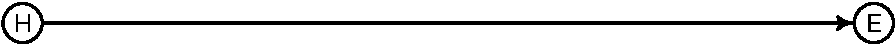
\includegraphics[width=0.5\linewidth,height=0.5\textheight]{ReplyToSteeleStefansson5_files/figure-latex/heDAG-prel-1} \end{center}

\noindent where \(H\) is the hypothesis node (upstream) and \(E\) the
evidence node (downstream). If an arrow goes from \(H\) to \(E\), the
full probability distribution associated with the Bayesian network is
defined by two probability tables.\footnote{A major point of contention
  in the interpretation of Bayesian networks is is the meaning of the
  directed arrows. They could be interpreted causally---as though the
  direction of causality proceeds from the events described by the
  hypothesis to event described by the evidence---but they need not be;
  see footnote \ref{footnote:causation}.} One table defines the prior
probabilities \(\pr{H=h}\) for all the states (or values) of \(H\), and
another table defines the conditional probabilities of the form
\(\pr{E=e \vert H=h}\), where uppercase letters represent the variables
(nodes) and lower case letters represent the states (or values) of these
variables. These two probability tables are sufficient to specify the
full probability distribution. The other probabilities---say \pr{E=e},
\pr{H=h \vert E=e}, etc.---follow by simply applying the probability
axioms. As nedded, more complex graphical structures can also be used.

Bayesian networks are relied upon in many fields, but have been rarely
deployed to model awareness growth (the exception is Williamson (2003)).
We think instead they are a good framework for this purpose. Awareness
growth can be modeled as a change in the graphical network---nodes and
arrows are changed, added or erased---as well as a change in the
probability distribution from the old to the new network. In this
section, we focus on cases of awareness expansion and turn to refinement
in the next section.

Recall the scenario \textsc{Friends} from before. It can be modeled with
the hypothesis-evidence idiom. The graph can be made more perspicuous by
labeling the downstream node `Behavior' (the evidence or fact to be
explained) and the upstream node `Reason' (the explanation or hypothesis
about the the cause of the behavior):

\begin{center}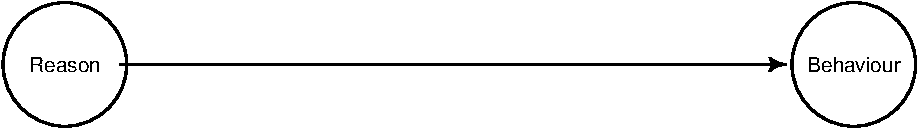
\includegraphics[width=0.5\linewidth,height=0.5\textheight]{ReplyToSteeleStefansson5_files/figure-latex/friendsDAG-1} \end{center}

\noindent Initially, before awareness growth, the hypothesis node
\textit{Reason} takes only two states: \textit{friends} and
\textit{affair}. These two states are meant to be exclusive and
exhaustive, so \textit{affair} functions as the negation of
\textit{friends}, and vice versa. After awareness growth---specifically,
awareness expansion---the two states are no longer exhaustive. A third
state is added: \textit{surprise}. So, in the formalism we are using,
expansion simply consists in the addition of an extra state to one of
the nodes of the network. The rest of the structure of the network
remains intact.

Recall that the ratio of posterior probabilities of \textit{friends} to
\textit{affairs} changed as a result of awareness expansion. The fact
that your partner and best fried met without telling you---call this
behavior \textit{secretive}---initially made \textit{affair} more likely
than \textit{friends}, but then the same fact made \textit{friends} more
likely than \textit{affair}. So, formally,
\[1>\frac{\pr{\textit{Reason=friends} \vert \textit{Behavior=secretive}}}{\pr{\textit{Reason=affair} \vert \textit{Behavior=secretive}}} < \frac{\ppr{+}{\textit{Reason=friends} \vert Behavior=secretive}}{\ppr{+}{\textit{Reason=affair} \vert \textit{Behavior=secretive}}}>1.\]
But, despite this change in posterior probabilities, it is plausible to
assume that the novel state added to the upstream node \textit{Reason}
did not change the relative plausibility of the two explanations
initially under consideration. Even after awareness expansion, the fact
that your partner and best fried met without telling
you---\textit{secretive}---makes better sense in light of
\textit{affair} compared to \textit{friends}:
\[\frac{\pr{\textit{Behavior=secretive} \vert \textit{Reason=affair}}}{\pr{\textit{Behavior=secretive} \vert  \textit{Reason=friends}}} = \frac{\ppr{+}{\textit{Behavior=secretive} \vert \textit{Reason=affair}}}{\ppr{+}{\textit{Behavior=secretive} \vert \textit{Reason=friends}}}>1.\]

\noindent This equality holds even though the novel explanation
\textit{surprise} introduced during awareness expansion makes better
sense of the secretive behavior overall:\footnote{Even though
  \(\frac{\ppr{+}{\textit{Behavior=secretive} \vert \textit{Reason=surprise}}}{\ppr{+}{\textit{Behavior=secretive} \vert \textit{Reason=affair}}}>1\)
  and
  \(\frac{\ppr{+}{\textit{Behavior=secretive} \vert \textit{Reason=affair}}}{\ppr{+}{\textit{Behavior=secretive} \vert \textit{Reason=friends}}}>1\)---so
  \textit{affair} still makes better sense of the evidence than
  \textit{friends} before and after awareness expansion---the posterior
  probability of \textit{friends} is higher than \textit{affair} after
  awareness expansion.}

\[\frac{\ppr{+}{\textit{Behavior=secretive} \vert \textit{Reason=surprise}}}{\ppr{+}{\textit{Behavior=secretive} \vert \textit{Reason=affair}}}>1. \]

This analysis suggests a slight reformulation of conditions such as
Reverse Bayesianism and Awareness Rigidity. Instead of comparing
posterior probabilities of hypotheses given the evidence
(\(\pr{H=h \vert E=e}\)), we can compare which explanation or hypothesis
makes better sense of the evidence (\(\pr{E=e \vert H=h}\)) So, for all
values \(e\) and \(h\) of upstream node \(H\) and downstream node \(E\)
in the old network, consider the following constraint:
\[\frac{\pr{E=e \vert H=h}}{\pr{E=e \vert H=h}} = \frac{\ppr{+}{E=e \vert H=h  \; \& \: X\neq x^*}}{\ppr{+}{E=e \vert H=h  \; \& \: X\neq x^*}}, \tag{C}\]
where \(x^*\) is the new state added and \(X\) is the node (upstream or
downstream) to which the new state belongs, such as
\(H=\textit{surprise}\) in \textsc{Friends}.

In words, the constraint says that one's old assessment of the relative
plausibility of two competing hypotheses in light of a fixed body of
evidence should remain unchanged after awareness expansion. Constraint
(C) is a variant of Reverse Bayesianism that only applies to conditional
probabilities of the form \(\pr{E=e \vert H=h}\) for Bayesian networks
of the form \(H \rightarrow E\). In addition, the constraint mimics
Awareness Rigidity in that it ensures that the conditional probabilities
in question exclude the novel state \(X=x^*\).

How generally does constraint (C) apply besides examples such as
\textsc{Friends}? The conjecture we are putting forward is that, so long
as there is no change in the structure of the network, the constraint
should hold. Since awareness expansion---as we have defined it---does
not involve any change in the structure, the constraint should hold for
all cases of expansion.\footnote{It is crucial that the new hypothesis
  or explanation does not change the existing structure of the network.
  For consider this example. You are wondering which horse will win the
  race. You have done a careful study of past performances under
  different conditions and concluded that Red is more likely to win than
  Green. But you have not considered the possibility that Grey would
  run. If Grey does run, it will have a greater chance of winning than
  the others, but will also make---for some odd reason---Green a much
  better racer than Red. So the odds that Green will win compared to Red
  should now be higher. Here, the new hypothesis introduces some novel
  informational that was not known before, say that the participation of
  Grey would weaken Red's performance and strengthen Green's
  performance. So the network should be changed in two ways: first, a
  new state should be added to the outcome node (Green wins, Red wins,
  Grey wins); and second, a new node should be added modeling the fact
  that Grey is participating and its participation affects Red's and
  Green's performance.}

\hypertarget{mathanis-examples}{%
\section{Mathani's Examples}\label{mathanis-examples}}

To acquire a firmer grasp on constraint (C), we now examine a couple of
examples by Mathani (2020). In her reading, these examples serve as
counterexamples to Reverse Bayesianism, but are also meant to challenge
the traditional distinction between expansion and refinement. But, when
modeled with Bayesian networks, they are straightforward cases of
awareness expansion.

The first of Matahani's examples goes like this:

\begin{quote}
\textsc{Tenant}: You are staying at Bob's flat which he shares with his landlord. You know that Bob is a tenant, and that there is only one landlord, and that this landlord also lives in the flat. In the morning you hear singing coming from the shower room, and you try to work out from the sounds who the singer could be. At this point you have two relevant propositions that you consider possible ... $landlord$ standing for the possibility that the landlord is the singer, and $bob$ standing for the possibility that Bob is the singer  \dots  Because you know that Bob is a tenant in the flat, you also have a credence in the proposition $tenant$ that the singer is a tenant. Your credence in $tenant$ is the same as your credence in $bob$, for given your state of awareness these two propositions are equivalent ... Now let's suppose the possibility suddenly occurs to you that there might be another tenant living in the same flat  ($other$).
\end{quote}

\doublespace

\noindent Initially, you thought the singer could either be the landlord
or Bob, the tenant. Then you come to the realization that a third person
could be the singer, another tenant. The possibility that there could be
a third person in the shower---besides Bob or the landlord---is a novel
explanation for why you hear singing in the shower. So \textsc{Tenant}
seems to be a standard case of expansion like \textsc{Friends}. At the
same time, this scenario is a bit more complicated. The expansion in
awareness goes along with an interesting conceptual shift. Before
awareness expansion, that Bob is in the shower and that a tenant is in
the shower are equivalent descriptions, but after the expansion, this
equivalence breaks down.

As Mathani shows, this scenario challenges Reverse Bayesianism. For it
is natural to assign \(1/3\) to \(landlord\), \(bob\) and \(other\)
after awareness growth, and 1/2 to \(landlord\) and \(bob\) before
awareness growth. That someone is singing in the shower is evidence that
someone must be in there, but without any more discriminating evidence,
each person should be assigned the same probability. Consequently, a
probability of 2/3 should be assigned to \(tenant\) after awareness
growth, but only 1/2 before. On this picture, the proportion of
\(landlord\) to \(tenant\) changes from 1:1 (before awareness growth) to
1:2 (after awareness growth).\footnote{ Here is more involved argument.
  Suppose, after you hear singing in the shower, you become sure someone
  is in there, but you cannot tell who. So
  \(\pr{landlord} = \pr{bob} = 1/2\), and since \(bob\) and \(tenant\)
  are equivalent, also \(\pr{tenant}\) = 1/2. Now, \(landlord\), \(Bob\)
  and \(tenant\) are all propositions that you were originally aware of,
  and thus Reverse Bayesianisn requires that their probabilities should
  remain in the same proportion after your awareness grows. But note
  that \(other\) entails \(tenant\) and \(bob\) and \(Other\) are
  disjoint, so it follows that \(\ppr{+}{other}\) must have zero
  probability. If \(\ppr{+}{other}\) were greater than zero, the
  proportion of of the probability of \(tenant\) to \(landlord\) (or the
  proportion of the probability of \(bob\) to \(landlord\)) should
  change.} \footnote{This scenario need not be a challenge for Awareness
  Rigidity. Much depends on the choice of the proposition \(T^*\) that
  picks out, from the vantage point of the new awareness state, the old
  possibility space prior to awareness growth. The proposition
  \(landlord \vee bob\) does the job. For
  \(\ppr{+}{landlord \vert landlord \vee bob}\) and
  \(\ppr{+}{bob \vert landlord \vee bob}\) should both equal \(1/2\),
  and thus \ppr{+}{other \vert landlord \vee bob}=0\$, but this does not
  mean that \(\ppr{+}{other \vert landlord \vee tenant}\) should equal
  zero. This is the intended result.}

But now recall that Reverse Bayesianism only applies to basic
propositions, which we defined earlier as propositions without
connectives. So a possible fix here is to adopt the following principle:
if two propositions happen to be equivalent relative to some awareness
state, they cannot be both considered basic. In \textsc{Tenant}, since
\(bob\) and \(tenant\) are initially equivalent descriptions of the same
state of affairs, they would not be considered both basic propositions.
If only \(bob\) is considered basic, along with \(landlord\), then the
proportion of the probability of \(bob\) and \(landlord\) would remain
the same during awareness growth, but not the proportion of the
probabilities of \(tenant\) and \(landlord\). This yields the intuitive
result. But it is odd that \(landlord\) would be considered basic, but
not \(tenant\). However, if \(tenant\) is considered basic along with
\(landlord\), Reverse Bayesianism would require that the proportion of
the probability of \(tenant\) and \(landlord\) remain the same during
awareness growth. This is counterintuitive.

So dividing propositions into basic and non-basic is riddled with
difficulties. But the above discussion alerted us to the fact that a
difference exists between propositions like \(bob\) and those like
\(tenant\). The latter describes a role that different people could play
besides Bob. Bayesian networks can help to model the person/role
distinction, as follows:

\begin{center}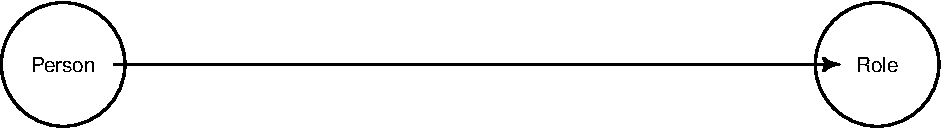
\includegraphics[width=0.5\linewidth,height=0.3\textheight]{ReplyToSteeleStefansson5_files/figure-latex/tenantsDAG-new-1} \end{center}

\noindent This subject-matter information---the distinction between
people and the role they play---remain fixed throughout the process of
awareness expansion. What changes is how the details are filled in.
Initially, the upstream node \(Person\) has two possible states,
representing who could be in the bathroom singing:
\textit{landlord-person} and \(bob\).\footnote{To simplify things, the
  assumption here is that the evidence of singing has already ruled out
  the possibility that no one would be in the shower. In principle, the
  network should be more complex and contain another node for the
  evidence to be explained (the fact of singing in the shower), as
  follows:
  \(\textit{Singing}\leftarrow\textit{Person}\rightarrow \textit{Role}\).}
The downstream node \(Role\) has also two values, \(landlord\) and
\(tenant\). After your awareness grows, the upstream node \(Person\)
should now have one more possible state, \(other\). Crucially, note that
since \textsc{Tenant} is a case of expansion by our definition---a state
was added to a node---constraint (C) should hold. This is precisely what
happens as illustrated in Table \ref{table:tenant}.\footnote{More
  generally, these conditional probabilities do not change during
  awareness growth:
  \[\pr{\textit{Role}=\textit{landlord} \vert \textit{Person}=\textit{landlord}}=
  \ppr{+}{\textit{Role}=\textit{landlord} \vert \textit{Person}=\textit{landlord}}\]
  \[\pr{\textit{Role}=\textit{landlord} \vert \textit{Person}=\textit{bob}}=
  \ppr{+}{\textit{Role}=\textit{landlord} \vert \textit{Person}=\textit{bob}}\]}
This is good news.

\begin{table}
\begin{tabular}{clccc}
&&&&\\
&&&&\\
$\pr{Role \vert Person}$ & & \multicolumn{3}{c}{$Person$} \\
 &   & \textit{landlord-person}  & \multicolumn{2}{c}{$bob$} \\
\multirow{2}{*}{$Role$} & $tenant$ & 0 & \multicolumn{2}{c}{1}\\
& $landlord$  & 1 & \multicolumn{2}{c}{0} \\
\hline
& \textsc{Total} & 1 & \multicolumn{2}{c}{1}  \\
\hline
\hline
$\ppr{+}{Role \vert Person}$ & & \multicolumn{3}{c}{$Person$} \\
&  & \textit{landlord-person} & $bob$ & $other$ \\
\multirow{2}{*}{$Role$} & $tenant$ & 0 & 1 & 1\\ 
& $landlord$ & 1 & 0 & 0 \\
\hline
& \textsc{Total} & 1 & 1 & 1  \\
\hline
\hline
$\pr{Person}$ & \multicolumn{2}{c}{$Person$} & \\
&  \textit{landlord-person} & $bob$ & \\
& 1/2 & 1/2 & \\
\hline
\hline
$\ppr{+}{Person}$ & \multicolumn{2}{c}{$Person$} & \\
&  \textit{landlord-person} & $bob$ & $other$ \\
& 1/3 & 1/3 & 1/3 \\
\end{tabular}
\caption{The table displays a plausible probability distribution for the \textsc{Tenant} scenarios. Constraint (C) is met.}
\label{table:tenant}
\end{table}

It is now time to test the tenability fo constraint (C) a bit further.
So far we only considered cases of awareness expansion in which a new
state was added to an \emph{upstream} node. In \textsc{Friends}, a state
was added to the upstream node \(Reason\), and in \textsc{Tenant}, a
state was added to the upstream node \(Person\). What if the new state
was added to a downstream node? For consider a variation of
\textsc{Friends}. Suppose that the downstream node \textit{Behavior}
could initially take only two values, say \textit{secretive} and
\textit{public}. You then realize the node could also take a third
value, say \textit{ambigous}. Initially, \textit{secretive} and
\textit{public} are considered exhaustive, but that is no longer true
after the addition of \textit{ambiguous}. So the old conditional
probabilities will change, specifically,
\(\pr{E=e \vert H=h}\neq \ppr{+}{E=e \vert H=h}\), where \(H\) is the
upstream node and \(E\) downstream. However, if we exclude the the novel
state, there should be no change, so
\(\pr{E=e \vert H=h \; \& \; E\neq e^* } = \ppr{+}{E=e \vert H=h \; \& \; E\neq e^*}\),
where \(e^*\) is the novel state added to the downstream node \(E\). So
constraint (C) should again be satisfied.

The same analysis applies to a more complex example by Mathani:

\begin{quote} 
\textsc{Coin}: You know that I am holding a fair ten pence UK coin which I am about to toss. You
have a credence of 0.5 that it will land $heads$, and a credence of 0.5 that it will
land $tails$. You think that the tails side always shows an engraving of a lion. So you
also  have a credence of 0.5 that it will land with the lion engraving face-up ($lion$): relative to your state of awareness $tails$ and $lion$ are equivalent.... Now let's suppose that you somehow become aware that occasionally ten pence coins have .... an engraving of Stonehenge on the tails side ($stonehenge$). 
\end{quote}

\doublespace

\noindent  The propositions \(tails\) and \(lion\) are equivalent prior
to awareness growth. Suppose you initially gave \(tails\) and \(lion\)
the same credence. If they are basic propositions, Reverse Bayesianism
would require that their relative proportions should stay the same after
awareness grow. The same is true of \(heads\) and \(tails\). But since
\(lion\) and \(stonehenge\) are incompatible and the latter entails
\(tails\), you should have \(\ppr{+}{stonehenge} = 0\), an undesirable
conclusion.

Mathani observes that this scenario blurs the distinction between
expansion and refinement. For one thing, \textsc{Coin} seems a case of
refinement. The space of possibiliiesy is held fixed---the coin could
come up heads or tails---but the options for tails are further refined,
for tails could be \(lion\) or \(stonehenge\). On the other hand, a new
possibility has been added after awareness growth, namely
\(stonehenge\), which had not been considered before. This would
indicate that \textsc{Coin} is a case of refinement. This ambiguity
makes it difficult to settle whether the scenario is a challenge for
Awareness Rigidity.\footnote{ If it is a case of refinement,
  \(heads \vee tails\) would pick out the entire possibility space even
  before awareness growth. If so, by Awareness Rigidity,
  \(\ppr{+}{tails \vert heads \vee tails}\) and
  \(\ppr{+}{lion \vert heads \vee tails}\) should both equal \(1/2\)
  since these were their probabilities before awareness growth. But
  these assignments would force
  \(\ppr{+}{stonehenge \vert heads \vee tails}\) to zero. To avoid this
  odd result for awareness Rigidity, one might argue that
  \(heads \vee tails\) picks out a possibility space larger than the old
  one, because it also includes the possibility of \(stonehenge\). So
  which is it?}

These difficulties disappear if the scenario is modeled using Bayesian
networks. The definition of awareness expansion we have been working
with is simple: whenever a new state is added to one of the nodes in the
network, awareness expansion takes place. The novel state can be added
to any node in the network. Each node, with its range of states,
characterizes an exhaustive partition of the possibility space. Whenever
a new state is added to a node, the partition associated with the node
expands. (Refinement, as we will see in the next section, consists in
the addition of a new node, not in the addition of a new state to an
existing node.)

By the definition of expansion just given, \textsc{Coin} counts as a
case of expansion, but it is structurally different from the more
straightforward cases such as \textsc{Friends} and \textsc{Tenant}.
Bayesian networks can help to model the difference precisely. The
scenario can be modeled by this familiar graph structure:

\begin{center}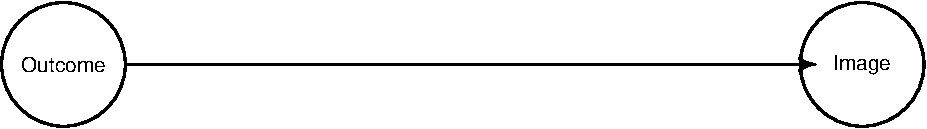
\includegraphics[width=0.5\linewidth,height=0.3\textheight]{ReplyToSteeleStefansson5_files/figure-latex/tailsDAG-1} \end{center}

\noindent The upstream node \(outcome\) has two states, \(tails\) and
\(heads\). These two states remain the same throughout. What changes are
the states associated with the \(imagine\) node downstream. Before
awareness growth, the node \(image\) has two states: \(lions\) and
\textit{heads-image}.\footnote{The heads side must have some image, not
  specified in the scenario.} You assume that \(Image=lions\) is true if
and only if \(Outcome=tails\) is true. Then, you come to the realization
that the imagines for tails could include a lion or a stonehenge
engraving. So, after awareness growth, the node \(Image\) contains three
states: \(lion\), \(stonehenge\) and \textit{heads-image}.

To some extent, \textsc{Coin} has the same structure as
\textsc{Tenant}---they are modeled by the same networks structure---but
there is also an important asymmetry that is apparent by comparing their
Bayesian networks. In the network for \textsc{Coin}, the states of the
upstream node remain fixed while a new state is added to the downstream
node. In the network for \textsc{Tenant}, the opposite happens: the
states of the downstream node remain fixed, while a new state is added
to the upstream node. Specifically, after awareness expansion, no new
state is added to upstream node \(Outcome\), but an additional state,
\(other\), is added to the downstream node \(Person\).

The states of the upstream node model what we tend to view---somewhat
loosely speaking--- as more causally fundamental compared to the states
of downstream nodes. In \textsc{Tenant}, who is the person singing in
the shower is more fundamental, while the proposition that describe
their roles are derivatives, for multiple people could play the same
role. In \textit{Coin}, that an outcome (heads or tails) could be
instantiated by different kinds of engravings is considered a derivative
fact. What seems causally fundamental is the type of outcome, not the
engraving. Bayesian networks offer a language to model these differences
that are crucial to model episodes of awareness expansion.

So what about constraint (C)? Plausible probability distributions for
the Bayesian networks associated with the scenario \textsc{Coin} is
displayed in Table \ref{table:coin}. It is easy to check that constraint
(C) is once again satisfied. So, the constraint has outperformed both
Reverse Bayesianism and Awareness Rigidity. But our objective here is
not to replace one formal constraint with another. As noted in the
introduction, we think that awareness growth cannot be modeled in a
purely formal matter. The success of constraint (C) relies on the right
network structure. How the networks should be built is based on our
subject-matter knowledge---for example, that people's behavior must have
a reason; that multiple peoples can play different roles; or that heads
and tails can be associated with different specific engravings. And
sometimes awareness growth may even require the very structure of the
network to change. This is our next topic.

\begin{table}
\begin{tabular}{clcc}
$\pr{Image \vert Outcome}$ & & \multicolumn{2}{c}{$Outcome$} \\
 &   & $heads$ & $tails$ \\
\multirow{2}{*}{$Image$} & $lion$ & 0 & 1\\
& \textit{heads-image} & 1 & 0 \\
\hline
& \textsc{Total} & 1 & 1 \\
\hline
\hline
$\ppr{+}{Image \vert Outcome}$ & & \multicolumn{2}{c}{$Outcome$} \\
&  & $heads$ & $tails$ \\
\multirow{3}{*}{$Image$} & $lion$ & 0 & 1/2\\ 
& $stonehenge$ & 0 & 1/2 \\
& \textit{heads-image} & 1 & 0 \\
\hline
& \textsc{Total} & 1 & 1 \\
\hline
\hline
$\pr{Outcome}=\ppr{+}{Outcome}$ & \multicolumn{2}{c}{$Outcome$} & \\
&  $heads$ & $tails$ & \\
& 1/2 & 1/2 & \\
\end{tabular}
\caption{Table displays a plausible probability distribution for the \textsc{Coin} scenario. Constraint (C) is met.}
\label{table:coin}
\end{table}

\hypertarget{refinement-with-bayesian-networks}{%
\section{Refinement with Bayesian
Networks}\label{refinement-with-bayesian-networks}}

\label{sec:structural-both}

We turn now from cases of awareness expansion to cases of awareness
refinement. The previous section illustrated why, when no change in
structure in the Bayesian network occurs, constraint (C) holds. But, of
course, awareness expansion may sometimes require to change the
structure of the network. What will happen to the constraint then? It
will likely fail, at least sometimes. The challenge is to develop a
method to determine when it holds and when it fails. This method will
afford us a firmer foundation for a general theory of awareness growth.

In the framework of Bayesian networks, expansion consists in adding
states to existing nodes in the network. Refinement, instead, can be
modeled by adding nodes to the network without adding any new state to
existing nodes. Intuitively, refinement takes place when an epistemic
agent acquires a more-fined grained picture of the situation, say
instead of thinking that the political spectrum is divided into liberals
and conservatives, the political spectrum can be further divided into
traditional-liberal, new-liberal, traditional-conservative and
new-conservative. The political spectrum is still divided into liberal
and conservative---no expansion occurred---but the two categories have
been further refined.\footnote{This example is from Pettigrew
  (forthcoming).}

Although there is no shortage of counterexamples to Reverse Bayesianism
when it comes to awareness refinement, we will use our own. Recall that
\textsc{Movies}---the refinement-based counterexample to Reverse
Bayesianism by Steele \& Stefánsson---suffered from a possible
objection. The example contained awareness refinement paired with a
standard case of Bayesian learning by conditionalization. Some might
argue that conditionalization, not awareness refinement, is responsible
for the change in probabilities. To alleviate this worry, we will work
with our own example which can be more clearly interpreted as mere
awareness refinement. Our own example will also allow us to underscore
the role of subject-matter assumptions in theorizing about awareness
growth. So consider this scenario:

\begin{quote}
\textsc{Lighting:} You have evidence that favors a certain hypothesis, say a witness 
saw the defendant around the crime scene. You give some weight to this evidence. 
In your assessment, that the defendant was seen around the crime scene (your evidence) raises the probability that the defendant was actually there (your hypothesis). But now you ask, what if it was dark when the witness saw the defendant? In light of your realization that it could have been dark, you wonder whether (and if so how) you should change the probability that you assigned to the hypothesis that the defendant was around the crime scene.
\end{quote}

As your awareness grows, you do not learn anything specific about the
lighting conditions, neither that they were bad nor that they were good.
You simply wonder what they were, a variable you had previously not
considered. So no Bayesian conditoning takes place in the strict sense,
although broadly speaking some new information has been
introduced.\footnote{The process of awareness growth in
  \textsc{Lighting} adds only one extra variable, lighting conditions,
  while \textsc{Movies} adds two extra variables, language difficulty
  and whether the owner is simple-minded or not. Further,
  \textsc{Movies} contains a clear-cut case of Bayesian updating, that
  the owner \emph{is} simple-minded. This is not so in
  \textsc{Lighting}. Strictly speaking, you are learning that it is
  \emph{possible} that the lighting conditions were bad. However, you
  are not conditioning on the proposition `the lighting conditions were
  bad' or `the lighting conditions were good'. So you are not learning
  about the lighting conditions in the sense of Bayesian updating.}
Something has changed in your epistemic state---you have a more
fine-grained assessment of what could have happened---but it is not
clear what you should do in this scenario. Since the lighting conditions
could have been bad but could also have been good, perhaps you should
just stay put until you learn something more specific.

In what follows, we illustrate how Bayesian networks helps to model what
is going on in \textsc{Lighting} and conclude that you should probably
revise downward your confidence in the hypothesis that the defendant was
around the crime scene. The starting point of our analysis is the usual
hypothesis-evidence idiom, repeated below for convenience:

\begin{center}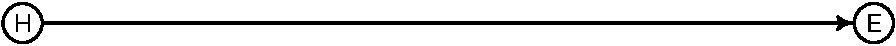
\includegraphics[width=0.5\linewidth,height=0.5\textheight]{ReplyToSteeleStefansson5_files/figure-latex/heDAG-1} \end{center}

\noindent Since you trust the evidence, you think that the evidence is
more likely under the hypothesis that the defendant was present at the
crime scene than under the alternative hypothesis:
\[\pr{\textit{E=seen} \vert \textit{H=present}} > \pr{\textit{E=seen} \vert \textit{H=absent}}\]
The inequality is a qualitative ordering of how plausible the evidence
is in light of competing hypotheses. No matter the numbers, by the
probability calculus, it follows that the evidence raises the
probability of the hypothesis \textit{H=present}.

Now, as you wonder about the lighting conditions, the graph should be
amended:

\begin{center}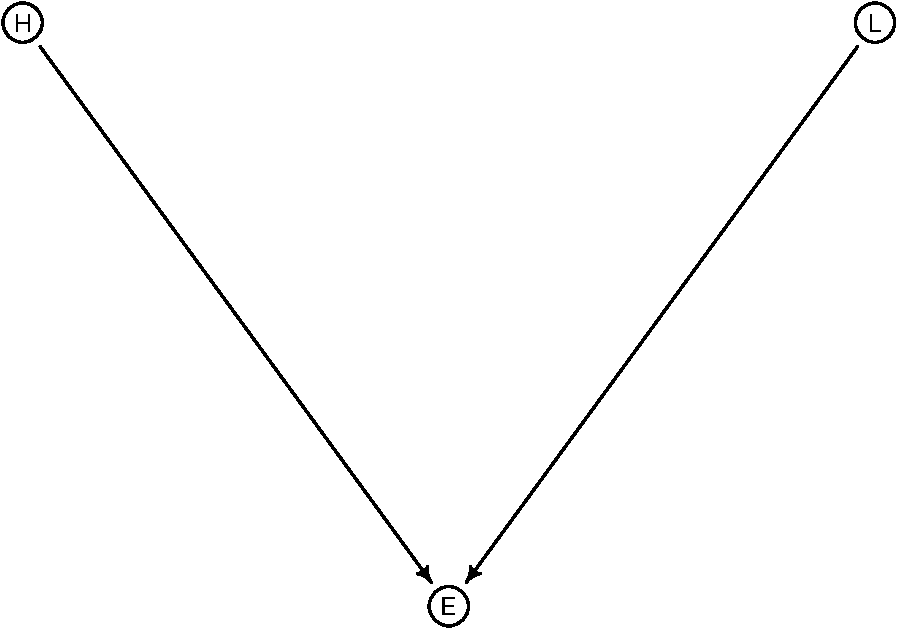
\includegraphics[width=0.5\linewidth,height=0.3\textheight]{ReplyToSteeleStefansson5_files/figure-latex/lighting2DAG-1} \end{center}

\noindent where the node \(L\) can have two values, \textit{L=good} and
\textit{L=bad}. Commonsense as well as psychological findings suggest
that when the visibility deteriorates, people's ability to identify
faces worsen. So a plausible way to modify your assessment of the
evidence is as follows:
\[\ppr{+}{\textit{E=seen} \vert \textit{H=present} \wedge \textit{L=good}} > \ppr{+}{\textit{E=seen} \vert \textit{H=absent} \wedge \textit{L=good}}\]
\[\ppr{+}{\textit{E=seen} \vert \textit{H=present} \wedge \textit{bad}} = \ppr{+}{\textit{E=seen} \vert \textit{H=absent} \wedge \textit{L=bad}}\]

\noindent In words, if the lighting conditions were good, you still
trust the evidence like you did before (first line), but if the lighting
conditions were bad, you regard the evidence as no better than chance
(second line). These probabilistic constraints are plausible, but should
ultimately be grounded on verifiable empirical regularities.

Despite the change in awareness, you have not learned anything in the
strict sense. Your new stock of evidence does not contain neither the
information that the lighting conditions were bad nor that they were
good. But the Bayesian network structure that represents your epistemic
state is now more fine-grained. The network contains the new variable
\(L\) which it did not contain prior to the episode of awareness growth.
In addition---and this is the crucial point---the new variable bears
certain \emph{structural relationships} with the variables \(H\) and
\(E\). The graphical network represents a direct probabilistic
dependency between the lighting conditions \(L\) and the witness sensory
experience \(E\), but does not allow for any direct dependency between
the lighting conditions and the fact that the defendant was (or was not)
at the crime scene. There is no direct arrow between the nodes \(L\) and
\(H\). This structure of dependencies captures our causal intuitions
about the scenario: the lighting conditions do affect what the witness
could see, but do not directly affect what the defendant might have
done.

Without Bayesian networks, episodes of awareness growth could only be
modeled by the addition of new propositions that were not previously in
the algebra. But this approach would fail to capture crucial
information. When awareness growth takes place against the background of
an intuitive causal structure of the world---as in the case of
\textsc{Lighting}---this structure should also be modeled. Bayesian
networks offer a formal framework that can do precisely that.

This model of causal structure can now guide us to decide whether the
restricted version of Reverse Bayesianism, what we called constraint
(C), holds in this scenario. Specifically, we need to assess whether the
following holds:
\[\frac{\pr{E=seen \vert H=present}}{\pr{E=seen \vert H=absent}}= \frac{\ppr{+}{E=seen \vert H=present}}{\ppr{+}{E=seen \vert H=absent}}.\]
The question here is whether you should assess the evidence at your
disposal---that the witness saw the defendant at the crime scene---any
differently than before.\footnote{Note that since no new state was added
  to an existing node, the condition \(X\neq x^*\) in constraint (C)
  (where \(x^*\) is the new state added to an existing node \(X\)) is
  redundant here.} As noted earlier, without a clear model of the
scenario, it might seem that you should simply stay put. After all,
besides the sensory experience of the witness, you have gained no novel
information about the lighting conditions. Should you thus conclude that
the evidence has the same value before and after the realization that
lighting could have been bad?

The evidence would have the same value if the likelihood ratios
associated with it relative to the competing hypotheses were the same
before and after awareness growth. But, in changing the probability
function from \(\pr{}\) to \(\ppr{+}{}\), it would be quite a
coincidence if this were true. In our example, many possible probability
assignments violate this equality. If before awareness growth you
thought the evidence favored the hypothesis \textit{H=present} to some
extent, after the growth in awareness, the evidence is likely to appear
less strong. To see this is tedious, so we relegate the details to a
footnote.\footnote{By the law of total probability, the right hand side
  of the equality in (C) should be expanded, as follows:
  \[\frac{\ppr{+}{E=e \vert H=h}}{\ppr{+}{E=e \vert H=h'}}=\frac{\ppr{+}{\textit{E=seen} \wedge \textit{L=good} \vert \textit{H=present}}+\ppr{+}{\textit{E=seen} \wedge \textit{L=bad} \vert \textit{H=present}}}{\ppr{+}{\textit{E=seen} \wedge \textit{L=good} \vert \textit{H=absent}}+\ppr{+}{\textit{E=seen} \wedge \textit{L=bad} \vert \textit{H=absent}}}.\]
  For concreteness, let's use some numbers:
  \[\pr{\textit{E=seen} \vert \textit{H=present}}=\ppr{+}{\textit{E=seen} \vert \textit{H=present} \wedge \textit{L=good}}=.8\]
  \[\pr{\textit{E=seen} \vert \textit{H=absent}}=\ppr{+}{\textit{E=seen} \vert \textit{H=absent} \wedge \textit{L=good}}=.4\]
  \[\ppr{+}{\textit{E=seen} \vert \textit{H=present} \wedge \textit{L=bad}} = \ppr{+}{\textit{E=seen} \vert \textit{H=absent} \wedge \textit{L=bad}}=.5.\]
  \[\ppr{+}{\textit{L=bad}} = \ppr{+}{\textit{L=good}}=.5.\] So the
  ratio
  \(\frac{\pr{\textit{E=seen} \vert \textit{H=present}}}{\pr{\textit{E=seen} \vert \textit{H=absent}}}\)
  equals \(2\). After the growth in awareness, the ratio
  \(\frac{\ppr{+}{\textit{E=seen} \vert \textit{H=present}}}{\ppr{+}{\textit{E=seen} \vert \textit{H=absent}}}\)
  will drop to \(\frac{.65}{.45}\approx 1.44\). The calculations here
  rely on the dependency structure encoded in the Bayesian network (see
  starred step below). \begin{align*}
  \ppr{+}{\textit{E=seen} \vert \textit{H=present}} &= \ppr{+}{\textit{E=seen} \wedge \textit{L=good} \vert \textit{H=present}}+\ppr{+}{\textit{E=seen} \wedge \textit{L=bad} \vert \textit{H=present}}\\
  &= \ppr{+}{\textit{E=seen} \vert \textit{H=present} \wedge \textit{L=good}}  \times \ppr{+}{\textit{L=good} \vert  \textit{H=present} }\\ & +\ppr{+}{\textit{E=seen}  \vert \textit{H=present} \wedge \textit{L=bad}} \times \ppr{+}{\textit{L=bad} \vert  \textit{H=present}}\\
  &=^* \ppr{+}{\textit{E=seen} \vert \textit{H=present} \wedge \textit{L=good}}  \times \ppr{+}{\textit{L=good}}\\ & +\ppr{+}{\textit{E=seen}  \vert \textit{H=present} \wedge \textit{L=bad}} \times \ppr{+}{\textit{L=bad}}\\
  &= .8 \times .5 +.5 *.5 = .65 
  \end{align*} \begin{align*}
  \ppr{+}{\textit{E=seen} \vert \textit{H=absent}} &= \ppr{+}{\textit{E=seen} \wedge \textit{L=good} \vert \textit{H=absent}}+\ppr{+}{\textit{E=seen} \wedge \textit{L=bad} \vert \textit{H=absent}}\\
  &= \ppr{+}{\textit{E=seen} \vert \textit{H=absent} \wedge \textit{L=good}}  \times \ppr{+}{\textit{L=good} \vert  \textit{H=absent} }\\ & +\ppr{+}{\textit{E=seen}  \vert \textit{H=absent} \wedge \textit{L=bad}} \times \ppr{+}{\textit{L=bad} \vert  \textit{H=absent}}\\
  &=^* \ppr{+}{\textit{E=seen} \vert \textit{H=absent} \wedge \textit{L=good}}  \times \ppr{+}{\textit{L=good}}\\ & +\ppr{+}{\textit{E=seen}  \vert \textit{H=absent} \wedge \textit{L=bad}} \times \ppr{+}{\textit{L=bad}}\\
  &= .4 \times .5 +.5 *.5 = .45 
  \end{align*} This argument can be repeated with many other numerical
  assignments.} If this is correct, constraint (C) has been violated.
Reverse Bayesianism is also violated since the ratio of the
probabilities of \textit{H=present} to \textit{E=seen}, before and after
awareness growth, has changed:
\[\frac{\ppr{\textit{E=seen}}{\textit{H=present}}}{\ppr{ \textit{E=seen}}{\textit{E=seen}}} \neq \frac{\ppr{+, \textit{E=seen}}{\textit{H=present}}}{\ppr{+, \textit{E=seen}}{\textit{E=seen}}},\]
where \(\ppr{\textit{E=seen}}{}\) and \(\ppr{+, \textit{E=seen}}{}\)
represent the agent's degrees of belief, before and after awareness
growth, updated by the evidence \(\textit{E=seen}\).\footnote{The
  scenario also violates Awareness Rigidity which requires that
  \(\ppr{+}{A \vert T^*}=\pr{A}\), where \(T^*\) corresponds to a
  proposition that picks out, from the vantage point of the new
  awareness state, the entire possibility space before the episode of
  awareness growth. In \textsc{Lighting}, however, \(T^*\) does not
  change, so Awareness Rigidity would require that
  \(\ppr{+}{A}=\pr{A}\), and instead in the scenario, we have
  \[\ppr{+}{\textit{H=present} \vert \textit{E=seen}} \neq \pr{\textit{H=present} \vert \textit{E=seen}}.\]}

The general lesson to be learned here has to do with the importance of
formalizing subject-matter assumptions and the role of Bayesian networks
in modeling awareness growth. Modeling the causal assumptions in
\textsc{Lighting} allowed us to see that constraint (C)---as well as
Reverse Bayesianism more generally---should fail here. But, as we noted
already, constraint (C) might hold in other, structurally different
cases of refinement. For consider this scenario:

\begin{quote}
\textsc{Veracity}: A witness saw that the defendant was around the crime
scene and you initially took this to be evidence that the defendant was
actually there. But then you worry that the witness might be lying or
misremembering what happened. Perhaps, the witness was never there, made
things up or mixed things up. Should you reassess the evidence at your
disposal? If so, how?
\end{quote}

\doublespace

\noindent   It might seem that this scenario is no different from
\textsc{Lighting}. The realization that lighting could be bad should
make you less confident in the truthfulness of the sensory evidence. And
the same conclusion should presumably follow from the realization that
the witness could be lying. But, upon closer scrutiny, things are not
that simple. To run the two scenarios together would be a mistake.

The evidence at your disposal in \textsc{Lighting} is the sensory
evidence---the experience of seeing---and the possibility of bad
lighting does affect the quality of your visual experience. So, if
lighting was indeed bad, this would warrant lowering your confidence in
the truthfulness of the visual experience. But the possibility of lying
in \textsc{Veracity} does not affect the quality of the visual
experience; it only affects the quality of the \textit{reporting} of
that experience. So, if the witness did lie, this would not warrant
lowering your confidence in the truthfulness of the visual experience,
only in the truthfulness of the reporting. The distinction between the
visual experience and its reporting is crucial here. Bayesian networks
help to model this distinction precisely, and then see why
\textsc{Lighting} and \textsc{Veracity} are structurally different.

The graphical network should initially look like the initial DAG for
\textsc{Lighting}, consisting of the hypothesis node \(H\) upstream and
the evidence node \(E\) downstream. As your awareness grows, the
graphical network should be updated by adding another node \(R\) further
downstream:

\begin{center}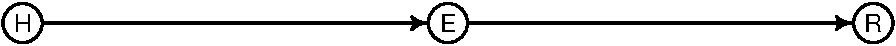
\includegraphics[width=0.5\linewidth,height=0.3\textheight]{ReplyToSteeleStefansson5_files/figure-latex/veracityDAG-1} \end{center}

\noindent As before, the hypothesis node \(H\) bears on the whereabouts
of the defendant and has two values, \textit{H=present} and
\textit{H=absent}. Note the difference between \(E\) and \(R\). The
evidence node \(E\) bears on the visual experience had by the witness.
The reporting node \(R\), instead, bears on what the witness reports to
have seen. The chain of transmission from `visual experience' to
`reporting' may fail for various reasons, such as lying or
misremembering.

In \textsc{Veracity}, the conditional probabilities,
\(\pr{E=e \vert H=h}\) should be the same as \(\ppr{+}{E=e \vert H=h}\)
for any values \(e\) and \(h\) of the variables \(H\) and \(E\) that are
shared before and after awareness growth. In comparing the old and new
Bayesian network, this equality falls out from their structure, as the
connection between \(H\) and \(E\) remains unchanged. Thus, constraint
(C) is perfectly fine in scenarios such as \textsc{Veracity}.

This does not mean that the assessment of the probability of the
hypothesis \textit{H=present} should undergo no change. If you worry
that the witness could have lied, this should presumably make you less
confident about \textit{H=present}. To accommodate this intuition,
\textsc{Veracity} can be interpreted as a scenario in which an episode
of awareness refinement takes place together with a form of retraction.
At first, after the learning episode, you update your belief based on
the \textit{visual experience} of the witness. But after the growth in
awareness, you realize that your learning is in fact limited to what the
witness \textit{reported} to have seen. The previous learning episode is
retracted and replaced by a more careful statement of what you learned:
instead of conditioning on \textit{E=seen}, you should condition on what
the witness reported to have seen, \textit{R=seen-reported}. This
retraction will affect the probability of the hypothesis
\textit{H=present}.

Where does this leave us? Refinement cases that might at first appear
similar can be structurally different in important ways, and this
difference can be appreciated by looking at the Bayesian networks used
to model them. In modeling \textsc{Veracity}, the new node is added
downstream, while in modeling \textsc{Lighting}, it is added upstream.
This difference affects how probability assignments should be revised.
Since the conditional probabilities associated with the upstream nodes
are unaffected, constraint (C) is satisfied in \textsc{Veracity}. By
contrast, since the conditional probabilities associated with the
downstream node will often have to change, the constraint fails in
\textsc{Lighting}.

This further corroborates our working hypothesis: subject-matter
assumptions---in the case of \textsc{Lighting} and \textsc{Veracity},
causal assumptions---about how we conceptualize a specific scenario are
the guiding principles about how we update the probability function
through awareness growth, not formal principles like Reverse
Bayesianism, Awareness Rigidity or even constraint (C).

\hypertarget{sure-no-gain-bets}{%
\subsection{Sure no-gain bets}\label{sure-no-gain-bets}}

Suppose the witness reports to have seeing the defendant around the
crime scene. You are not aware that the witness could be lying. Thus,
you are 100\% confident that the witness saw is what they report to have
seeing. In fact, you make no distinction between reporting to have
seeing and seeing itself. So you would be willing to buy for 1\$ the
following bet: if the witness saw the defendant, you get 1\$, and 0\$
otherwise. If the witness did see the defendant, you get you 1\$ back,
and otherwise you loose \textbackslash1\$. You are 100\% sure the
witness did see the defendant, so---by your lights---you stand to loose
no money whatsoever from this bet. But suppose that, as a matter of
fact, there is a difference between reporting and seeing. So,the witness
might report to have seeing something without actually having seeing it.
So, contrary to your conviction, that the witness saw the defendant is
not 100\% probable. This means that you would be willing to engage in a
bet in which you are guaranteed not to win any money and could
potentially lose money. If the witness did see the defendant you would
get your 1\$ back, but if not, you would lose it.

\hypertarget{towards-a-general-theory}{%
\section{Towards a general theory}\label{towards-a-general-theory}}

We conclude with some programmatic remarks. We think that the awareness
of agents grows while holding fixed certain material structural
assumptions, based on commonsense, semantic stipulations or causal
dependency.\footnote{Arrows in Bayesian networks are often taken to
  represent causal relationships, but other interpretations exist.
  Schaffer (2016) discusses an interpretation in which arrows represent
  grounding relations rather than causality. \label{footnote:causation}}
To model awareness growth, we need a formalism that can express these
material structural assumptions. This can done using Bayesian networks,
and we offered some illustrations of this strategy. These material
assumptions also guide us in formulating the adequate conservative
constraints, and these will inevitably vary on a case-by-case basis. The
literature on awareness growth from a Bayesian perspective is primarily
concerned with a formal, almost algorithmic solution to the problem.
Insofar as Reverse Bayesianism is an expression of this formalistic
aspiration, we agree with Steele and Stefánsson that we are better off
looking elsewhere.

Awareness growth can occur in different ways. The key question is to
what extent probability assignments that were made prior to the episode
of awareness growth can be retained. There seems to no clear rule that
can decide that. We propose the following procedure. Construct a
Bayesian network prior to awareness growth and compare it with the new
Bayesian network after awareness growth. If the new arrows and nodes are
all downstream, the old probabilities table should not be changed. The
paradigmatic cases of this are scenarios \textsc{Veracity} and
\textsc{Coin}. If, instead, the new arrows and and nodes are upstream,
the old probabilities tables should be changed. The paradigmatic
examples are \textsc{Lighting} and \textsc{Tenant}.

\singlespace

\hypertarget{references}{%
\section*{References}\label{references}}
\addcontentsline{toc}{section}{References}

\hypertarget{refs}{}
\begin{CSLReferences}{1}{0}
\leavevmode\vadjust pre{\hypertarget{ref-bradley2017}{}}%
Bradley, R. (2017). \emph{Decision theory with a human face}. Cambridge
University Press.

\leavevmode\vadjust pre{\hypertarget{ref-chihara1987}{}}%
Chihara, C. S. (1987). Some problems for bayesian confirmation theory.
\emph{British Journal for the Philosophy of Science}, \emph{38}(4),
551--560.

\leavevmode\vadjust pre{\hypertarget{ref-eerman1992}{}}%
Earman, J. (1992). \emph{Bayes or bust? A critical examination of
bayesian confirmation theory}. MIT press.

\leavevmode\vadjust pre{\hypertarget{ref-fenton2013GeneralStructureLegal}{}}%
Fenton, N., Neil, M., \& Lagnado, D. A. (2013). A {General Structure}
for {Legal Arguments About Evidence Using Bayesian Networks}.
\emph{Cognitive Science}, \emph{37}(1), 61--102.
\url{https://doi.org/10.1111/cogs.12004}

\leavevmode\vadjust pre{\hypertarget{ref-glymour1980}{}}%
Glymour, C. (1980). \emph{Theory and evidence}. Princeton University
Press.

\leavevmode\vadjust pre{\hypertarget{ref-howson1976}{}}%
Howson, C. (1976). The development of logical probability. In
\emph{Essays in memory of imre lakatos. Boston studies in the philosophy
of science} (pp. 277--298). Springer.

\leavevmode\vadjust pre{\hypertarget{ref-karniViero2015}{}}%
Karni, E., \& Vierø, M.-L. (2015). Probabilistic sophistication and
reverse bayesianism. \emph{Journal of Risk and Uncertainty Volume},
\emph{50}, 189--208.

\leavevmode\vadjust pre{\hypertarget{ref-lakatos1968}{}}%
Lakatos, I. (1968). Changes in the problem of inductive logic.
\emph{Studies in Logic and the Foundations of Mathematics}, \emph{51},
315--417.

\leavevmode\vadjust pre{\hypertarget{ref-mathani2020}{}}%
Mathani, A. (2020). Awareness growth and dispositional attitudes.
\emph{Synthese}, \emph{198}(9), 8981--8997.

\leavevmode\vadjust pre{\hypertarget{ref-Pettigrew2022}{}}%
Pettigrew, R. (forthcoming). How should your beliefs change when your
awareness grows? \emph{Episteme}, 1--25.
\url{https://doi.org/10.1017/epi.2022.33}

\leavevmode\vadjust pre{\hypertarget{ref-roussos2021}{}}%
Roussos, J. (2021). Awareness growth and belief revision.
\emph{Manuscript}.

\leavevmode\vadjust pre{\hypertarget{ref-schaffer2016}{}}%
Schaffer, J. (2016). Grounding in the image of causation.
\emph{Philosophical Studies}, \emph{173}, 49--100.

\leavevmode\vadjust pre{\hypertarget{ref-steeleStefansson2021}{}}%
Steele, K., \& Stefánsson, O. (2021). Belief revision for growing
awareness. \emph{Mind}, \emph{130}(520), 1207--1232.

\leavevmode\vadjust pre{\hypertarget{ref-wenmackersRomeijn2016}{}}%
Wenmackers, S., \& Romeijn, J.-W. (2016). New theory about old evidence:
A framework for open-minded bayesianism. \emph{Synthese Volume},
\emph{193}, 1225--1250.

\leavevmode\vadjust pre{\hypertarget{ref-williamson2003}{}}%
Williamson, J. (2003). Bayesianism and language change. \emph{Journal of
Logic, Language, and Information}, \emph{12}(1), 53--97.

\leavevmode\vadjust pre{\hypertarget{ref-zabell1992}{}}%
Zabell, S. (1992). Predicting the unpredictable. \emph{Synthese},
\emph{90}(1), 205--232.

\end{CSLReferences}

\end{document}
